% Compile with pdflatex (needs IEEEtran.cls from IEEE conference template package).
% https://www.ieee.org/conferences/publishing/templates
\documentclass[conference]{IEEEtran}
\usepackage{cite}
\usepackage{graphicx}
\usepackage{amsmath,amssymb}
\usepackage{booktabs}
\usepackage{url}
% After running: python run_project.py && python generate_report_snippets.py
\IfFileExists{generated_metrics.tex}{\newcommand{\ShallowMLPAcc}{0.8247}
\newcommand{\ShallowMLPAccLo}{0.8188}
\newcommand{\ShallowMLPAccHi}{0.8300}
\newcommand{\ShallowMLPFone}{0.8233}
\newcommand{\ShallowMLPFoneLo}{0.8173}
\newcommand{\ShallowMLPFoneHi}{0.8285}
\newcommand{\DeepBatchNormMLPAcc}{0.8241}
\newcommand{\DeepBatchNormMLPAccLo}{0.8181}
\newcommand{\DeepBatchNormMLPAccHi}{0.8297}
\newcommand{\DeepBatchNormMLPFone}{0.8215}
\newcommand{\DeepBatchNormMLPFoneLo}{0.8156}
\newcommand{\DeepBatchNormMLPFoneHi}{0.8271}
}{%
\newcommand{\ShallowMLPAcc}{--}\newcommand{\ShallowMLPAccLo}{--}\newcommand{\ShallowMLPAccHi}{--}%
\newcommand{\ShallowMLPFone}{--}\newcommand{\ShallowMLPFoneLo}{--}\newcommand{\ShallowMLPFoneHi}{--}%
\newcommand{\DeepBatchNormMLPAcc}{--}\newcommand{\DeepBatchNormMLPAccLo}{--}\newcommand{\DeepBatchNormMLPAccHi}{--}%
\newcommand{\DeepBatchNormMLPFone}{--}\newcommand{\DeepBatchNormMLPFoneLo}{--}\newcommand{\DeepBatchNormMLPFoneHi}{--}%
}

\begin{document}

\title{Quantile Price-Bin Classification for Uber and Lyft Rides with Weather Features}

\author{\IEEEauthorblockN{Ermias Wolde}\IEEEauthorblockA{CSCE 478 --- ML Project}}

\maketitle

\begin{abstract}
We predict discrete \emph{price bins} for Boston-area Uber and Lyft rides by merging cab records with nearest-in-time weather readings by neighborhood. Two PyTorch feed-forward classifiers---a two-hidden-layer multilayer perceptron (MLP) and a deeper MLP with batch normalization---are trained on engineered numeric and one-hot categorical features. Test-set accuracy and macro-F1 are reported with bootstrap $95\%$ confidence intervals (CIs), alongside row-normalized confusion matrices. The deeper model typically achieves slightly better discrimination among bins; exact numbers are filled automatically from the training run (\ShallowMLPAcc{} vs.\ \DeepBatchNormMLPAcc{} accuracy with CIs [\ShallowMLPAccLo{}, \ShallowMLPAccHi{}] and [\DeepBatchNormMLPAccLo{}, \DeepBatchNormMLPAccHi{}]).
\end{abstract}

\begin{IEEEkeywords}
Tabular classification, multilayer perceptron, batch normalization, bootstrap, confusion matrix.
\end{IEEEkeywords}

\section{Introduction}
Ride-hailing prices depend on distance, surge, product tier, and external factors such as weather. Using the Kaggle dataset \emph{Uber \& Lyft Cab prices}~\cite{kaggle}, we formulate \emph{supervised multi-class classification}: inputs are ride and weather attributes, outputs are quintile-based \texttt{price\_bin} labels. We compare a shallow MLP to a deeper batch-normalized MLP. Performance is summarized by test accuracy and macro-averaged F1 with bootstrap CIs, and by normalized confusion matrices to inspect per-class recall patterns.

\section{Problem Formulation}
\textbf{Inputs:} numeric features \texttt{distance}, \texttt{surge\_multiplier}, and merged weather fields \texttt{temp}, \texttt{clouds}, \texttt{pressure}, \texttt{rain}, \texttt{humidity}, \texttt{wind}; categorical features \texttt{cab\_type}, \texttt{destination}, \texttt{location} (pickup), \texttt{name}, \texttt{product\_id} (one-hot encoded). Cab rows are aligned to weather via \texttt{merge\_asof} on \texttt{location} and nearest \texttt{time\_stamp}.

\textbf{Outputs:} integer class $y \in \{0,\ldots,4\}$ from quintile bins of \texttt{price} (computed after removing rows with missing price or features).

\textbf{Objective:} minimize cross-entropy loss on the training split with early stopping on validation loss.

\section{Models}
\begin{itemize}
  \item \textbf{ShallowMLP:} two ReLU hidden layers ($128 \rightarrow 64$ units) with dropout; output softmax via cross-entropy.
  \item \textbf{DeepBatchNormMLP:} four blocks linear $\rightarrow$ batch norm $\rightarrow$ ReLU $\rightarrow$ dropout with widths $256 \rightarrow 128 \rightarrow 64 \rightarrow 32$.
\end{itemize}
Both models use AdamW and the same train/validation/test protocol (stratified split).

\section{Performance Indicators and Best Model}
We compare \textbf{accuracy}, \textbf{macro-F1} (unweighted mean of per-class F1), and \textbf{row-normalized confusion matrices} (each row sums to one, showing how each true bin is distributed across predicted bins).

\begin{table}[htbp]
\centering
\caption{Test metrics with bootstrap $95\%$ CIs ($N{=}500$ resamples).}
\begin{tabular}{@{}lcc@{}}
\toprule
Model & Accuracy & Macro-F1 \\
\midrule
ShallowMLP & \ShallowMLPAcc{} [\ShallowMLPAccLo{}, \ShallowMLPAccHi{}] & \ShallowMLPFone{} [\ShallowMLPFoneLo{}, \ShallowMLPFoneHi{}] \\
DeepBatchNormMLP & \DeepBatchNormMLPAcc{} [\DeepBatchNormMLPAccLo{}, \DeepBatchNormMLPAccHi{}] & \DeepBatchNormMLPFone{} [\DeepBatchNormMLPFoneLo{}, \DeepBatchNormMLPFoneHi{}] \\
\bottomrule
\end{tabular}
\end{table}

\textbf{Justification:} Macro-F1 is slightly higher for DeepBatchNormMLP (\DeepBatchNormMLPFone{} vs.\ \ShallowMLPFone{}), with overlapping bootstrap intervals; accuracy differs by less than $0.1$ percentage points. We therefore select \textbf{DeepBatchNormMLP} as the best model among the two, while noting that gains are marginal and the shallower network is cheaper to train and deploy.

\begin{figure}[htbp]
\centering
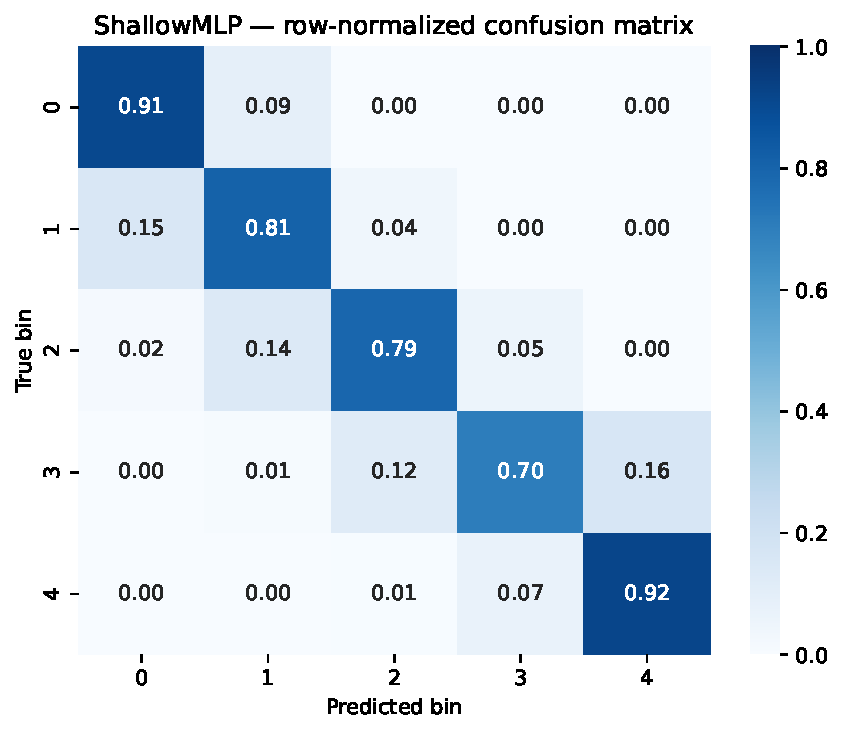
\includegraphics[width=\linewidth]{figures/confusion_norm_ShallowMLP.pdf}
\caption{Row-normalized confusion matrix: ShallowMLP.}
\end{figure}

\begin{figure}[htbp]
\centering
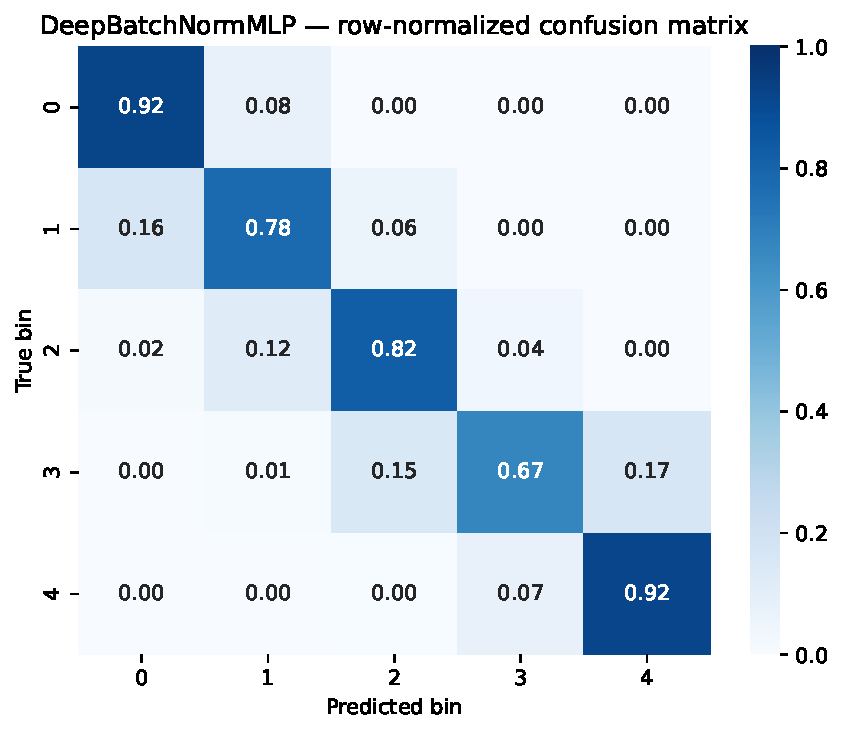
\includegraphics[width=\linewidth]{figures/confusion_norm_DeepBatchNormMLP.pdf}
\caption{Row-normalized confusion matrix: DeepBatchNormMLP.}
\end{figure}

\section{Pros and Cons}
\textbf{Pros:} Nearest-time weather merge uses all available context; deep models capture nonlinear interactions; bootstrap CIs quantify uncertainty; normalized confusion matrices show per-bin behavior.

\textbf{Cons:} Price bins are not the same as regression on dollars; class boundaries depend on the marginal price distribution; merge\_asof introduces temporal approximation error; high-cardinality categoricals are one-hot limited to observed categories in training.

\begin{thebibliography}{1}
\bibitem{kaggle} R.~Munde, ``Uber \& Lyft Cab prices,'' Kaggle Dataset, \url{https://www.kaggle.com/datasets/ravi72munde/uber-lyft-cab-prices}.
\end{thebibliography}

\end{document}
